\section{Sensitivity and Robustness}
\noindent\rule[\linienAbstand]{\linewidth}{\linienDickeDick}

\subsection{Residual Analysis}
\noindent\rule[\linienAbstand]{\linewidth}{\linienDicke}
The graphical tools Tukey-Anscombe plot, scale-location plot and q-q plot which check goodness of fit for the simple linear regression model can also be used for multiple linear regression models.\\
In addition to the Tukey-Anscombe plots mentioned above the \emph{Residuals vs. Leverage plot} is introduced which will be discussed in the next section.\\

In multiple regression, it is no longer clear which explanatory variable might cause a deficit. To find out graphically, the residuals $e = y - \hat{y}$ are plotted versus an explanatory variable $x_k$ used as the horizontal axis instead of the fitted values $\hat{y}$.\\

\subsection{Influential Observations}
\noindent\rule[\linienAbstand]{\linewidth}{\linienDicke}
The answer to the question whether an observation is an outlier depends on the model. If outliers remain in the data, the question arises of how strongly they influence the analysis.\\
Influence diagnostics is based on the idea to remove one observation, repeat the analysis and measure the change. \textbf{Cook’s distance measure} is a very popular influence diagnostic tool which measures the change of the fitted values if one observation $i$ is omitted.
\begin{equation}
  d_i = \frac{(\hat{\textbf{y}}_{(-1)} - \hat{\textbf{y}})^t(\hat{\textbf{y}}_{(-1)}-\hat{\textbf{y}})}{p \hat{\sigma}^2}
\end{equation}
where $p = m + 1$ is the number of estimated parameters in the case of a model with intercept and $p = m$ in the case without intercept.\\
Fortunately it is not necessary to repeat the analysis $n$ times. A mathematical simplification leads to the equivalent form
\begin{equation}
  d_i = \frac{\tilde{e}_{std,i}^2}{p}\frac{h_{ii}}{1-h_{ii}}
\end{equation}
Cook’s distance measure is a function of the $i$th standardised residual $\tilde{e}_{std,i}$ and the so-called leverages $h_{ii}$ of the $i$th observation. The leverages
\begin{equation}
  h_{ii} = \textbf{H}_{ii} = (\textbf{X}(\textbf{X}^t\textbf{X})^{-1}\textbf{X}^t)_{ii}
\end{equation}
are the diagonal entries of the hat matrix $\textbf{H}$. Leverages $h_{ii}$ satisfy $0 \geq h_{ii} \geq 1$ and the mean of all leverages is always $\frac{p}{n}$.\\

Interpretation of leverages:
\begin{itemize}
  \item A large leverage $h_{ii}$ has a big influence on the fitted values.
  \item A large leverage $h_{ii}$ reduces the variance of the $i$th residual, and therefore the $i$th observation is close to regression line (hyper-plane).
  \item Leverage is a measure of how far away the explanatory values of an observation are from those of the other observations.
\end{itemize}

When is an observation a leverage point?\\
\textbf{Rule of thumb:} Observations are dangerous if\\
\begin{equation}
  h_{ii} > 2 \frac{p}{n}
\end{equation}

\textbf{Huber's classification:}\\ Observations with
\begin{itemize}
  \item $h_{ii} \leq 0.2$ are harmless.
  \item $ 0.2 < h_{ii} < 0.5$ are potentially dangerous.
  \item $0.5 < h_{ii}$ should be avoided.
\end{itemize}

\textbf{Rule of thumb for Cook's distance measure:}
\begin{itemize}
  \item If $d_i > 1$ then the ith observation is dangerous.
  \item If $d_i \leq 1$ then the ith observation is harmless.
\end{itemize}


\begin{table}[H]
  \setlength{\tabcolsep}{0.2em}
  \scriptsize
  \begin{tabular}{p{\linewidth / 2 - 0.5em}@{\hskip 1em}p{\linewidth / 2 - 0.5em}}
    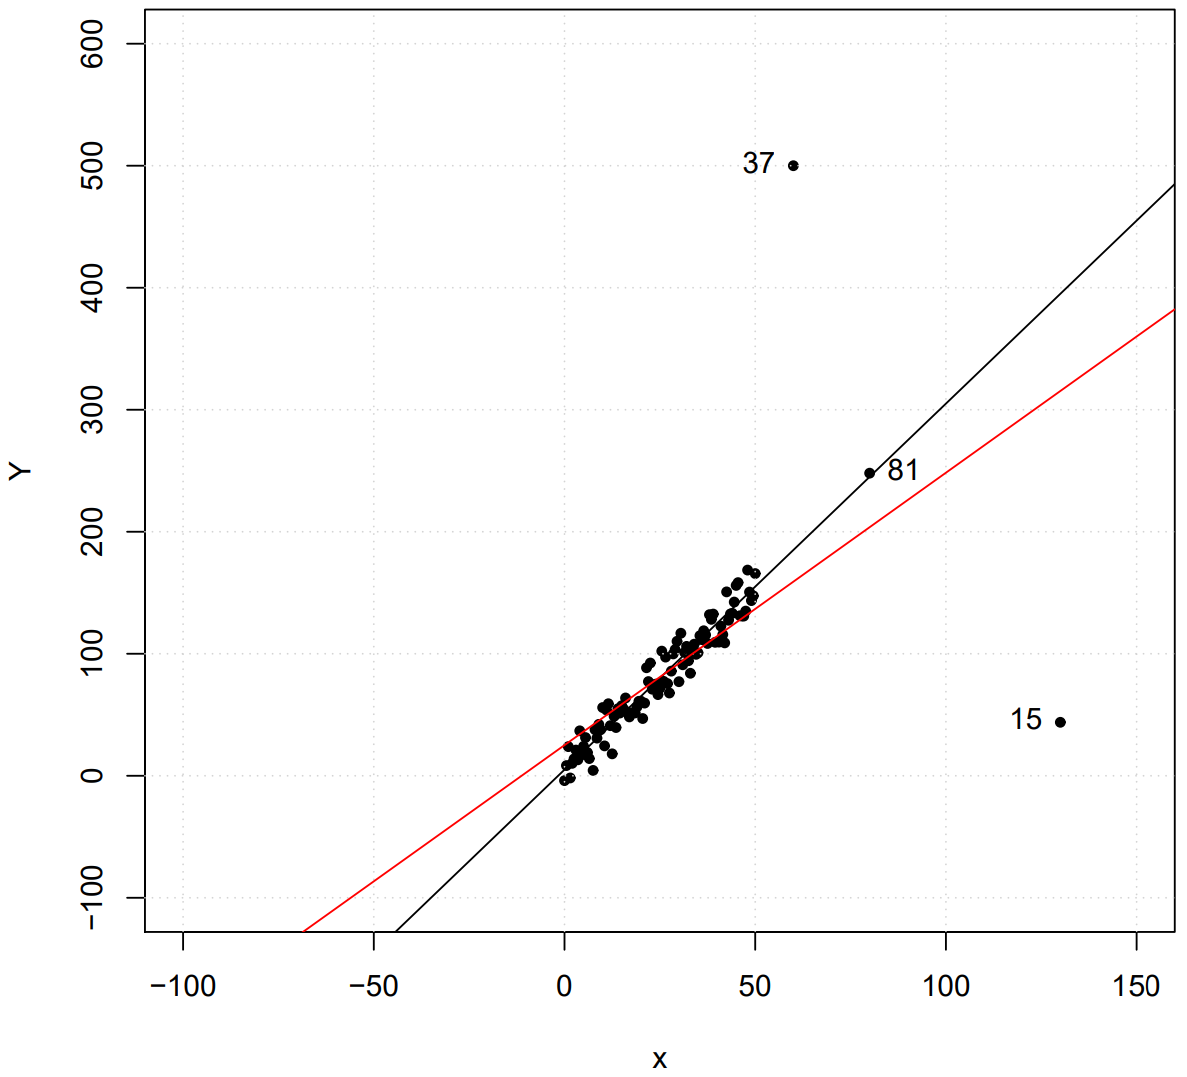
\includegraphics[width=\linewidth]{Pics/10.2.3.png}& 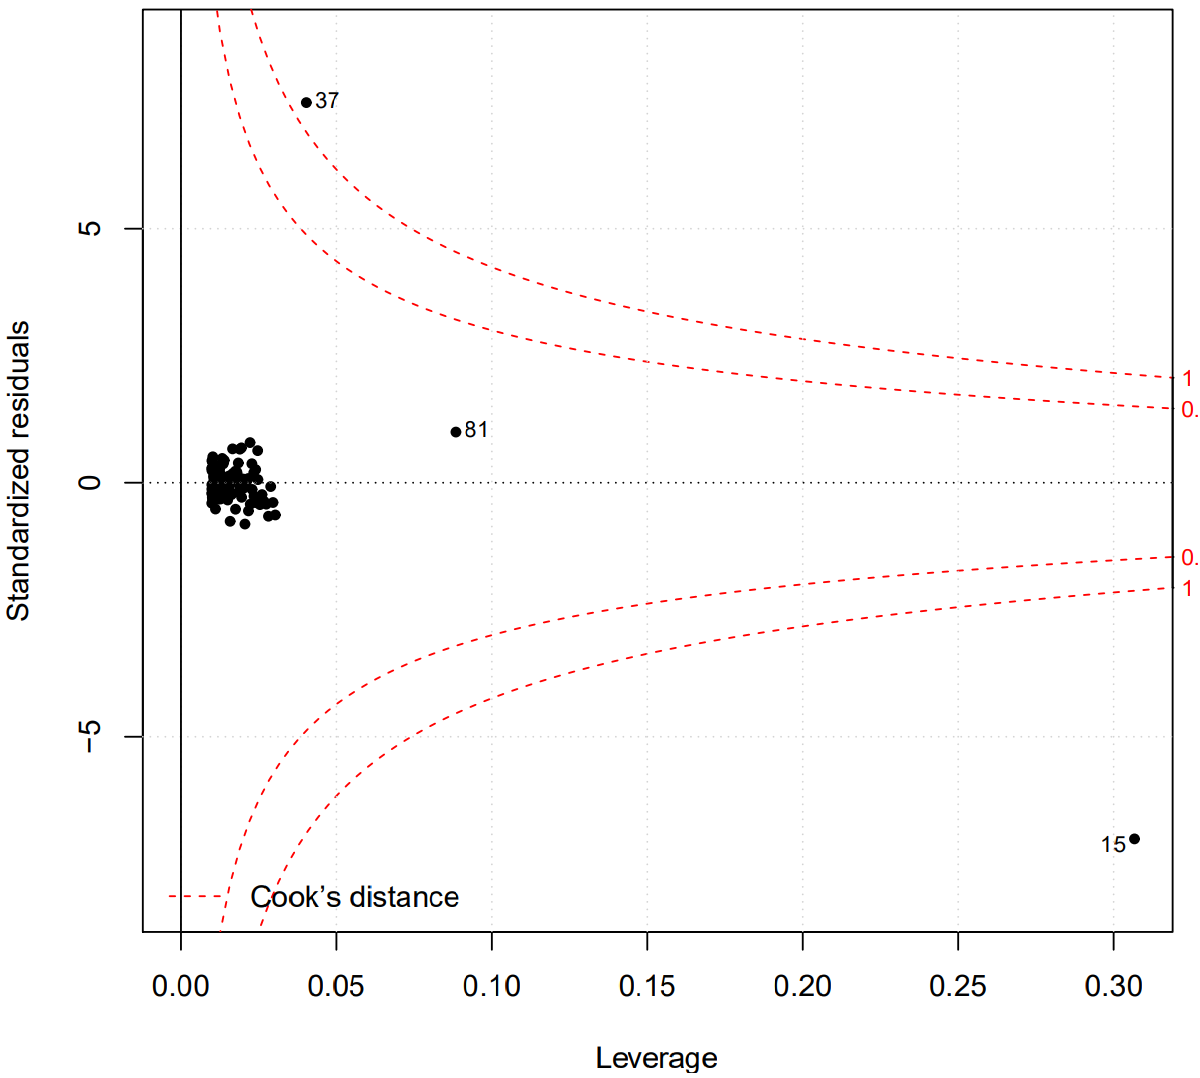
\includegraphics[width=\linewidth]{Pics/10.2.4.png} \\
    Artificial data with two outliers. Original model (black) and estimated best fit (red). &
    Standardised residuals versus leverages with two outliers. Contours of Cook’s distance measure (red).\\
  \end{tabular}
\end{table}

\subsection{Weighted linear regression}
\noindent\rule[\linienAbstand]{\linewidth}{\linienDicke}
It certainly makes sense to give greater weight to the observations with smaller random error. That is, the more precise observations gain weight in the statistical analysis.\\
Therefore we need to find the least-squares estimate for weighted multiple regression.\\
we want to find the vector of least-squares estimators $\beta$, which minimise

\begin{equation}
  S(\mathbf{\beta}) = \sum^n_{i = 1}w_i\varepsilon^2_i) = \varepsilon^t \mathbf{W} \varepsilon =
  (\mathbf{y}-\mathbf{X}\mathbf{\beta})^t \mathbf{W}(\mathbf{y}-\mathbf{X}\mathbf{\beta})
\end{equation}

which simplifies to the so-called weighted least-squares normal equations
\begin{equation}
  \mathbf{X}^t\mathbf{Wy} = \mathbf{X}^t\mathbf{WX}\hat{\pmb{\beta}}
\end{equation}

The solution of the normal equations is the least-squares estimator
\begin{equation}
  \hat{\pmb{\beta}} = (\mathbf{X}^t\mathbf{WX})^{-1} \mathbf{X}^t\mathbf{Wy}
\end{equation}


\subsection{Robust Methods}
\noindent\rule[\linienAbstand]{\linewidth}{\linienDicke}
The goal of robust statistics is to find parameter estimates as if the outliers did not exist\\

The robustness of an estimator can be investigated by two measures: the influence function and the breakdown point. Both measures are based on the idea of studying the effect of an estimator under the influence of gross errors, i.e. arbitrary added data.

\textbf{Breakdown Point}\\
The breakdown point is the minimal proportion of incorrect observations which cause completely unrealistic estimates.\\
\textbf{Gross Error Sensitivity}\\
The gross error sensitivity is based on the influence function and measures the maximum effect of a single observation on the estimated value.\\

\textbf{Robust Regression M-Estimator}\\
The influence of an outlier in observation $i$ is manifested in a large residual $e_i$. Therefore, the main idea of robust regression is to introduce weights $w_i$ which weigh down this influence. If we want to limit the influence of large residuals the function
\begin{equation}
  \Psi(e) = w_i e_i
\end{equation}
must be limited. This can be achieved, for instance by the Hubert's $\psi$ -function.
\begin{figure}[H]
  \centering
  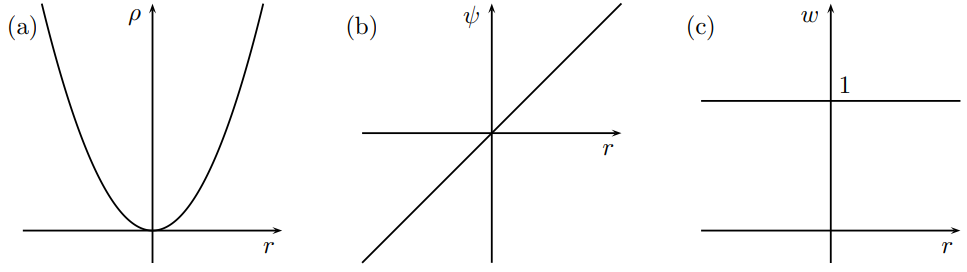
\includegraphics[width=\linewidth]{Pics/10.4.1.png}
  \caption{Loss function $\rho$ of least-squares estimate (a), $\psi$-function (b) and corresponding weight function $w$ (c).}
\end{figure}
\begin{figure}[H]
  \centering
  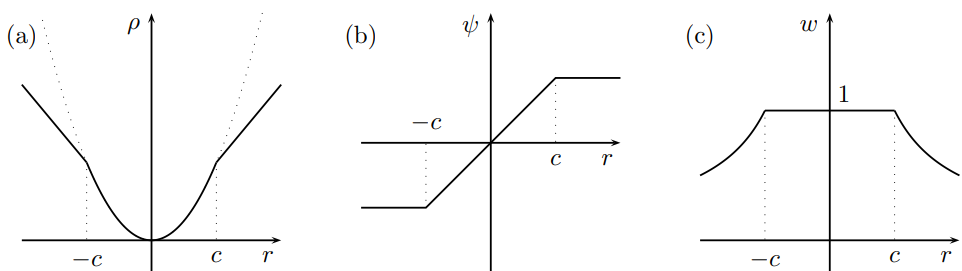
\includegraphics[width=\linewidth]{Pics/10.4.2.png}
  \caption{Loss function $\rho$ (a) of Huber’s $\psi$-function (b) and corresponding weight function $w$ (c).}
\end{figure}
The corresponding weights are then simply
\begin{equation}
  w_i = \frac{\psi (e_i)}{e_i}
\end{equation}
The threshold $c$ in Huber’s $\psi$-function is set to be $c = 1.345$ which is based on theoretical efficiency considerations.\\
The regression M-estimation limits only the influence of large residuals, but is still prone to leverage points and therefore has a break point of zero. To be able to handle bad leverage points we need a redescending $\psi$-function such that observations with large absolute residuals are gradually ignored.\\

\textbf{Modified Robust Regression M-Estimator}\\
\begin{figure}[H]
  \centering
  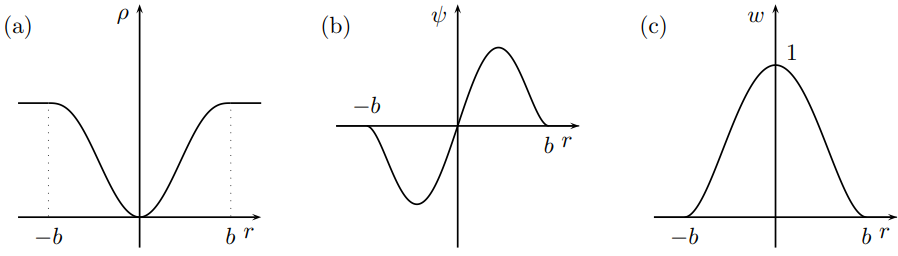
\includegraphics[width=\linewidth]{Pics/10.4.5.png}
  \caption{Loss function $\rho$ (a) of Tukey's bisquare $\psi$-function (b) and corresponding weight function $w$ (c).}
\end{figure}
The threshold $b$ of Tukey’s bisquare is set to be $b = 4.685$ which is based on theoretical efficiency considerations. The regression MM-estimator has a breakdown point of $\frac{1}{2}$ and an efficiency and an asymptotic distribution like the regression M-estimator.
